\DiaryEntry{First Order Differential Equations (I)}{2018-05-11}{ODE}

Taken from "Exploring Differential Equations".


\subsubsection{Constant Coefficients}

We consider

\bee
y' - ay = 0 \equiv \frac{dy(t)}{dt} - ay(t) = 0, \quad y(0) = y0
\eee

We can use separation of variables to obtain

\bee
\frac{dy(t)}{y(t)} = a dt \rightarrow \ln y(t) = at + C \rightarrow y(t) = ce^{at}
\eee

where $c = e^C$ is constant which needs to adapted to the initial conditions. In case $a>0$, the derivative $y'$ has the same sign as $y$. So for $y(t) > 0$, the derivative is also positive and therefore $y(t)$ will increase further. For $y(t) < 0$, the derivative is negative and $y(t)$ will decrease further. These increases and decreases follow the exponential function.

In case of negative $a<0$, the signs of $y$ and $y'$ are reversed: If $y(t)$ is positive, it will decrease, therefore reducing the derivative and therefore, the decrease is slowing, until $y(t)$ becomes asymptotically zero. In case of negative $y(t)$, $y(t)$ will increase with slowing speed, until it also becomes asymptotically zero.


The following plot shows two solutions with different initial conditions for the ODE $y'+y=0$ (i.e., $a>0$). Note the exponential blow-up of the curves.

\begin{figure}[H]
	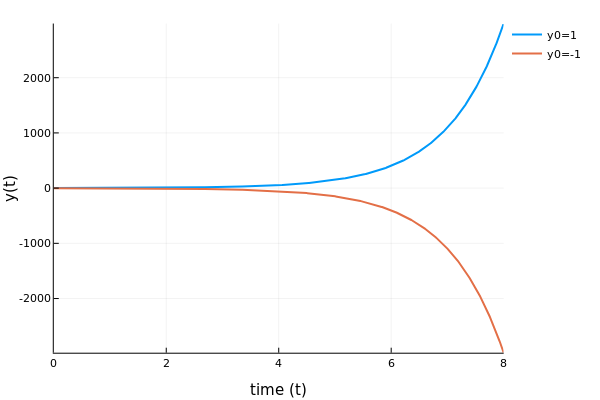
\includegraphics[scale=0.5]{images/ode_01_01.png}
\end{figure}



The following plot shows two solutions with different initial conditions for the ODE $y'+y=0$ (i.e., $a<0$)

\begin{figure}[H]
	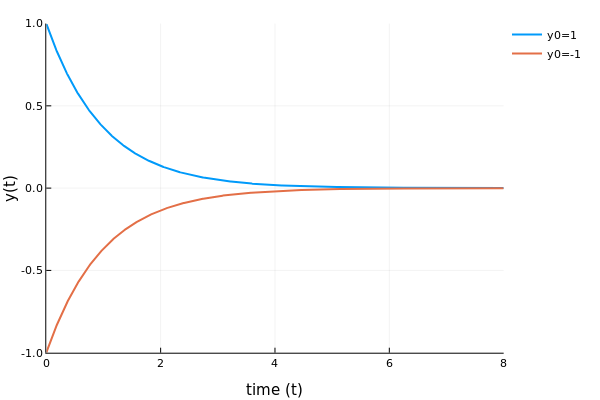
\includegraphics[scale=0.5]{images/ode_01_02.png}
\end{figure}


\subsubsection{Non-constant Coefficients}

Above principles allow understanding what happens when the ODE coefficient $a$ is allowed to vary; either time-varying (i.e. $y'(t)-a(t)y(t) = 0$) or depending on $y$ (i.e. $y'(t)-a(y)y(t) = 0$).

Consider the ODE

\bee
y'(t) + \cos(y)y = 0, \quad y(0) = y0
\eee

Solutions for several initial values are shown in the following Figure.

\begin{figure}[H]
	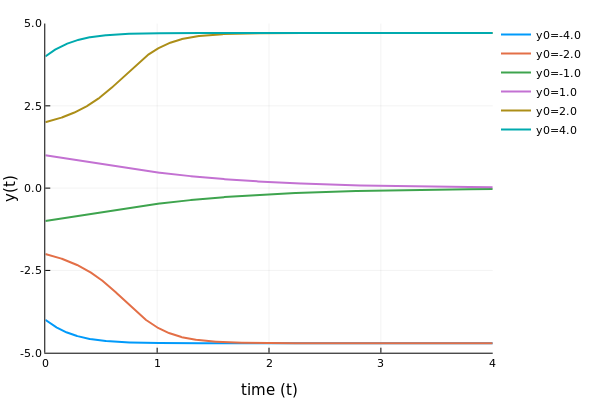
\includegraphics[scale=0.5]{images/ode_01_03.png}
\end{figure}

Since $|\cos| \leq 1$, there is no exponential blow-up; however, depending on the initial value $y(0)$, the ODEs arrive at different asymptotic solutions. This can be explained by plotting the phase-plane; a plot $y'$ vs $y$ which is in the following Figure.

\begin{figure}[H]
	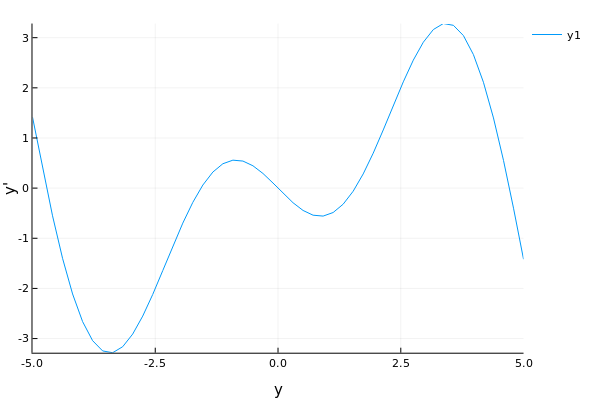
\includegraphics[scale=0.5]{images/ode_01_04.png}
\end{figure}

Let's start with $y(0) = 1$ first: From the phase plot it can be seen that $y'(0) < 0$, therefore $y(t)$ starts decreasing. Although $y'$ becomes smaller, it does not change sign, and therefore $y \rightarrow 0$ asymptotically.

For an initial value $y(0) = 2$, the derivative $y'>0$ and therefore $y$ increases. The rate of increase is at maximum at $y \approx 3.5$, and then becomes slower. The derivative becomes zero at $y \approx 4.7$, that's the value $y(t)$ approaches for large $t$. Apart from the zeros, $y'$ takes on larger values for large $y$ (because of its form $\cos(y) y$) - so larger initial values tend to converge to their fixed point faster.

For quantitative results, we calculate the zeros of $y\cos(y)$:

\bee
y\cos(y) = 0 \rightarrow y = 0, y = \pm \pi/2, y = \pm 3\pi/2
\eee

This shows that initial values $y(0) \in [-\pi/2; \pi/2] = [-1.57; 1.57]$ arrive at the fixed point $y(\infty)=0$. The next interval is $[\pi/2; 3\pi/2] = [1.57;4,71]$: Initial values in this interval arrive at the fixed point $y(\infty)=4.71$. The pattern continues for the other intervals...


As an example for ODEs with time-varying coefficients consider

\bee
y'(t) - \sin(t^2) y(t) = 0
\eee

A plot of the solution for $y(0) = 1$ and the function $\sin(t^2)$ can be seen in the following Figure.

\begin{figure}[H]
	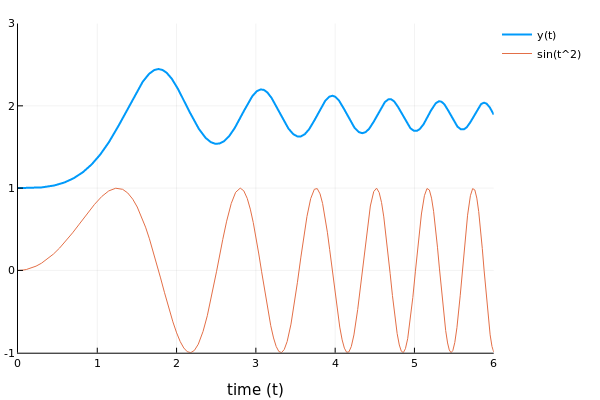
\includegraphics[scale=0.5]{images/ode_01_05.png}
\end{figure}

Here the interplay between time intervals with $a>0$ and increasing $y(t)$ and intervals with $a<0$ and decreasing $y(t)$ can be seen clearly. The "coefficient" changes faster with increasing time and this effect can also be seen on $y(t)$: It also changes faster for larger $t$ and the amplitude becomes smaller, because $y(t)$ cannot follow fast enough.

Separation of variables yields the following expression for $y(t)$:

\bee
\frac{dy}{y(t)} = \sin(t^2)dt \rightarrow y(t) = c \exp \left( \int_{u=0}^t \sin(u^2) du \right)
\eee

I don't know, whether this can be solved in closed form. \qed


The general problem of ODEs with time-varying coefficients has the following form

\bee
y'(t) - a(t)y(t) = 0 \rightarrow \frac{dy(t)}{dt} = a(t)y(t)
\eee

We can separate variables again, integrate both sides and obtain

\bee
\ln y(t) = \int_{s=0}^t a(s) ds + C \rightarrow y(t) = c \exp \left( \int_{s=0}^t a(s) ds \right) \qed
\eee